% \begin{frame}{Problem}
%   % Notes: Spend around 30 sec on this slide
%   \centering
%   \begin{figure}
%     
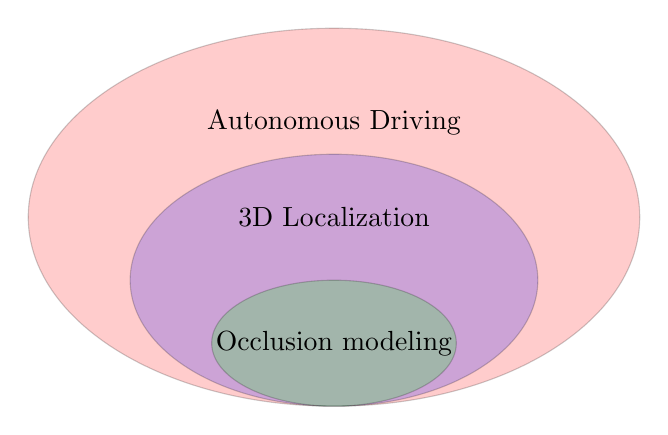
\begin{tikzpicture}[	venn circle/.style={opacity=0.2,fill=#1,draw}]
  %\path[use as bounding box, draw] (-3*1.618, -3) rectangle (3*1.618, 3);

\path[venn circle=red] (0,0) ellipse (3*1.618 and 3);
\node at (0, 1.5) {Autonomous Driving};
\path[venn circle=blue] (0, -1) ellipse (2*1.618 and 2);
\node at (0, 0) {3D Localization};
\path[venn circle=green] (0, -2) ellipse (1.2* 1.618 and 1);
\node at (0, -2) {Occlusion modeling};
\end{tikzpicture}

%   \end{figure}
% \end{frame}
% This slide doesn't make it clear what problem we are trying to solve?  May be
% the slide that Manmohan made with an example image with cars and detections
% is better

% Should we have introduction slide that highlights our contributions?
% but we should have contributions to highlight them. Contributions are perhaps
% better with positive results but still. I don't think we should have negative
% results as a surprise. (It won't as they would have read the report.)

\begin{frame}{Problem}
  % Need a flowchart that describes the input and desired output of the system
 \tikzset{/tikz/x=0.8cm,/tikz/y=0.8cm}
 \newlength{\units}
 \setlength{\units}{0.8cm}
  \scriptsize{
    
\begin{tikzpicture}[
    every edge/.style = {very thick,>=stealth,draw,red,->},
    data/.style = {ellipse,fill=blue!20,draw,
    minimum width=3\units},
    algo/.style = {rectangle,rounded corners,fill=red!20,draw}]
  \coordinate (hgap) at (3.5, 0);
  \coordinate (vgap) at (0, -1);
  \coordinate (o) at (0,0);
  \path 
  ($(o)+2*(vgap)$) node[data] (mv) {Mono-Video}
  ++($1.5*(vgap)$) node[data] (gps) {GPS}
  +($(vgap)$) node[data] (map) {Map};

  \path 
  ($(o) + (hgap)$) node[data] (det) {Detections}
  +(vgap) node[data] (pt) {Point Tracks}
  +($2*(vgap)$) node[data] (gp) {Ground plane}
  +($3*(vgap)$) node[data] (ego) {Egomotion}
  +($4*(vgap)$) node[data] (lane) {Lanes};


  \begin{pgfonlayer}{background}
    % Left-top corner of the background rectangle
    \path (det.east |- det.north)+(0.25,0.25) node (a) {};
    % Right-bottom corner of the background rectanle
    \path (mv.west |- map.south)+(-0.25,-0.25) node (c) {};
    % Draw the background
    \path[fill=green!20,rounded corners, draw=green,thick]
    (a) rectangle (c);
    \node at ($(det) - (hgap)$) {Inputs};
  \end{pgfonlayer}

  \path 
  ($(mv)+2*(hgap)$) node [algo] (os) {Our system}
  +($(hgap)$) node [data,text width=2.5\units] (out) {3D localization and dimensions};

 %\path[use as bounding box,draw] (map.south west) rectangle ($(out.east |- det.north)+(0.25,0.25)$);



  \path (mv) edge (det);
  \path (mv) edge (pt);
  \path (mv) edge (gp);
  \path (mv) edge (ego);
  \path (mv) edge (lane);
  \path (gps) edge (lane);
  \path (map) edge (lane);

  \path (det) edge (os);
  \path (pt) edge (os);
  \path (gp) edge (os);
  \path (ego) edge (os);
  \path (lane) edge (os);

  \path (os) edge (out);
\end{tikzpicture}

  }
\end{frame}

% \begin{frame}{Problem}
%   \visible<-1>{
%     \begin{tikzpicture}
%       \node[anchor=south west,inner sep=0] (image) at (0,0)
%       {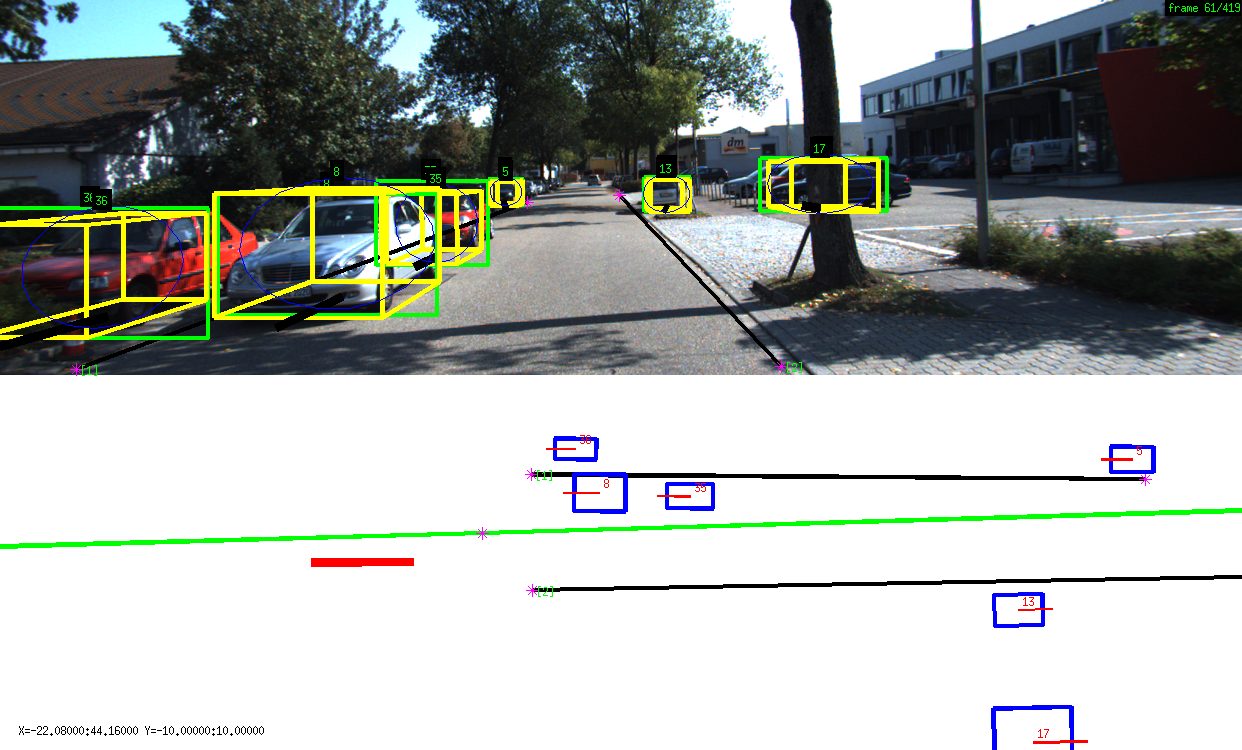
\includegraphics[width=\textwidth]{graphics/0000000061_bevdown.png}};
%       \fill[color=white] (image.south west) rectangle (image.east);
%     \end{tikzpicture}
%   }
% \end{frame}
\begin{frame}{Problem}

  \def\arrow{
    (0,0) -- ++(1,0)
    -- ++(0,1) -- ++(0.3, 0)
    -- ++(-0.8, 1) -- ++(-0.8, -1) -- ++(0.3, 0) -- ++(0, -1) }

  \begin{tikzpicture}
    \node[anchor=south west,inner sep=0] (image) at (0,0)
    {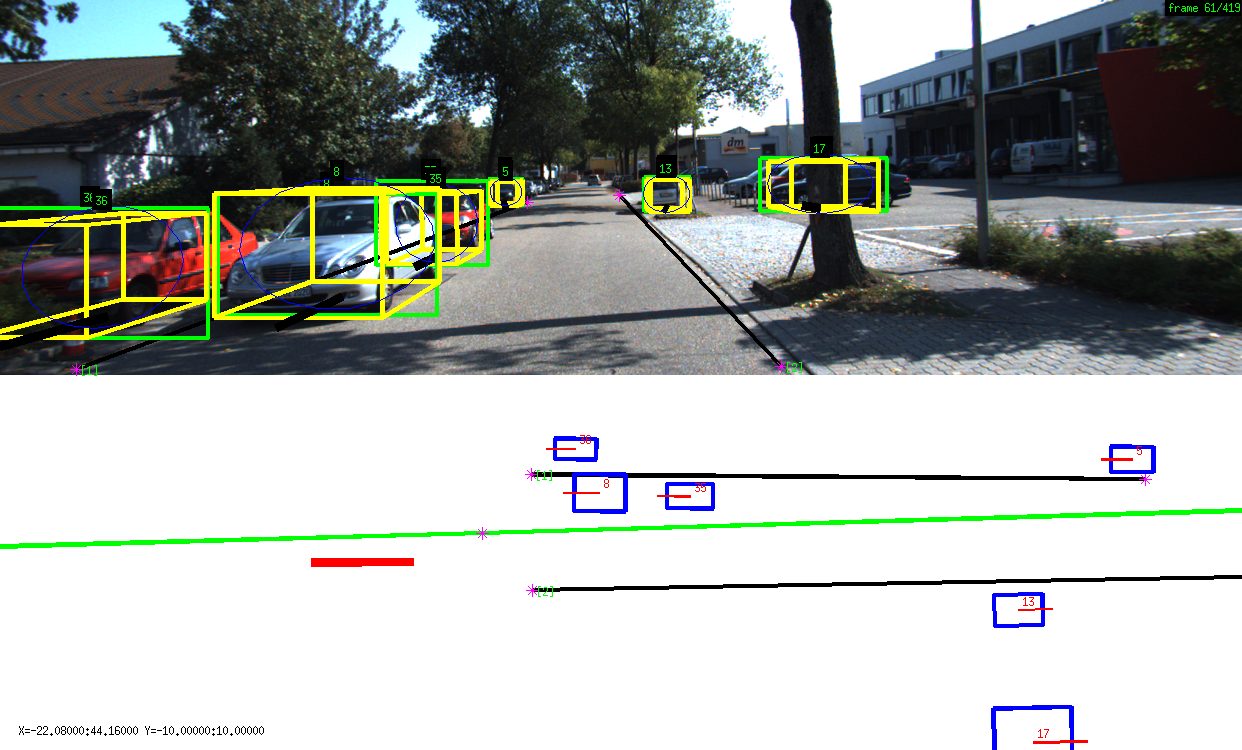
\includegraphics[width=\textwidth]{graphics/0000000061_bevdown.png}};
    \begin{scope}[x={(image.south east)},y={(image.north west)}]
      \fill[color=red,scale=0.05,shift={(10,11)},rotate=180,]\arrow;
    \end{scope}
  \end{tikzpicture}
\end{frame}
